\section{Задача}

\begin{frame}
	\frametitle{Постановка задачи о конвекции}

	\begin{minipage}{0.35\linewidth}
		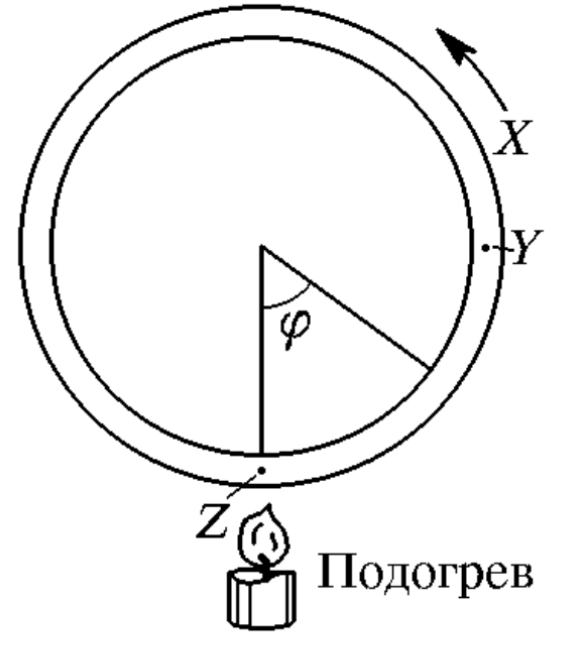
\includegraphics[width = 1\linewidth]{img/knot.png}
	\end{minipage}
	\hfill
	\begin{minipage}{0.55\linewidth}
		Зарождение квазипериодических потоков можно пронаблюдать на примере задачи о конвекции в замкнутой петле.

		При достаточно большой интенсивности подогрева возможно возникновение конвекционного течения в трубе.
	\end{minipage}
	
\end{frame}

\begin{frame}
	\frametitle{Метод решения}
	Ограничившись разложением уравнения $T(\varphi)$ в ряд Фурье только до первой гармоники:
	$$T(\varphi) = T_0(1 + Y \sin \varphi + Z \cos \varphi)$$

	Исходя из качественных соотношений составим уравнения для динамических переменных $X, Y, Z$, подставляя их в выражение для $T(\varphi)$, получим их в виде.

	$$\dot{X} = c Y - \beta X,  \hspace{1cm} \dot{Y} = X Z - D Y, \hspace{1cm} \dot{Z} = A - X Y - D Z$$
\end{frame}

\begin{frame}
	\frametitle{Пояснения}

	Предположим, что имеет место течение с постоянной скоростью, $\dot{\varphi} = X$. Тогда можно записать:		$$T = f(\varphi - X t) = T_0(1 + Y \sin (\varphi - X t) + Z \cos(\varphi - X t))$$

	Введя обозначение $\varphi' = \varphi - X t$:
	$$\dot{T} = T_0(Y \dot{\varphi}' \cos \varphi' - Z \dot{\varphi}' \sin{\varphi'}) = T_0(- X Y \cos \varphi' + Z X \sin \varphi').$$
\end{frame}

\begin{frame}
	\frametitle{Решение}

	Далее, производя замену переменных для уравнений для $X, Y, Z$:
	$$X = D x, \hspace{1cm} Y = \frac{\beta D y}{c}, \hspace{1cm} Z = -\frac{\beta D z}{c}, \hspace{1cm} t = D t,$$
	получаем уравнения Лоренца:
	$$\dot{x} = \sigma(y-x), \hspace{1cm} \dot{y} = r x - y -x z, \hspace{1cm} \dot{z} = -b z + x y$$
	решение которых сводится к решению системы дифференциальных уравнений.
\end{frame}

\begin{frame}
	\frametitle{Исследование решения}

	Промоделируем полученное решение с помощью $\textit{Python}$.
	\centering
	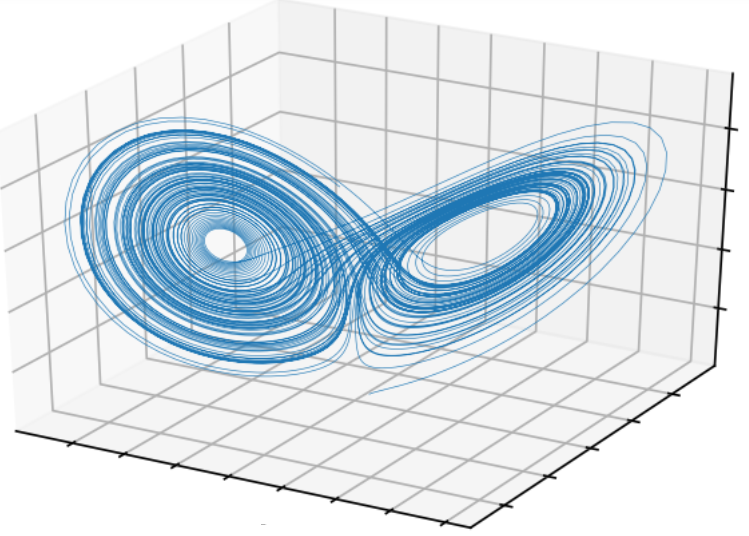
\includegraphics[height = 0.45\linewidth]{img/attr_L.png}
\end{frame}	

\begin{frame}
	Также в проекции на каждую ось действительно наблюдается хаотичное поведение.

	\centering
	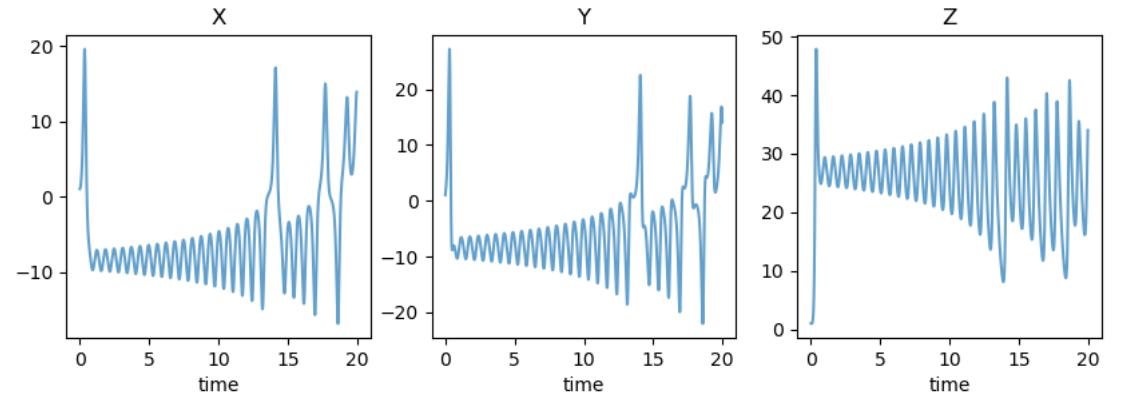
\includegraphics[width = 0.95\linewidth]{img/xyz.png}
\end{frame}

\begin{frame}
	\frametitle{Механическая аналогия}

	Так называемое Водяное колесо Лоренца имеет в своей сущности чисто механические уравнения, однако их решения сводится всё к той же системе уравнений Лоренца.

	\centering
	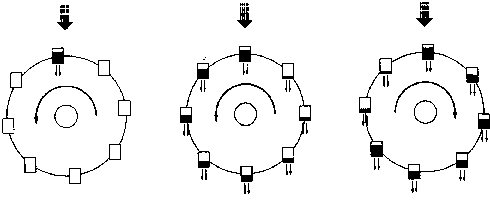
\includegraphics[width = 0.8\linewidth]{img/whaterwheel.png}
\end{frame}

\begin{frame}
	\frametitle{Неудавшийся эксперимент}

	\begin{minipage}{0.35\linewidth}
		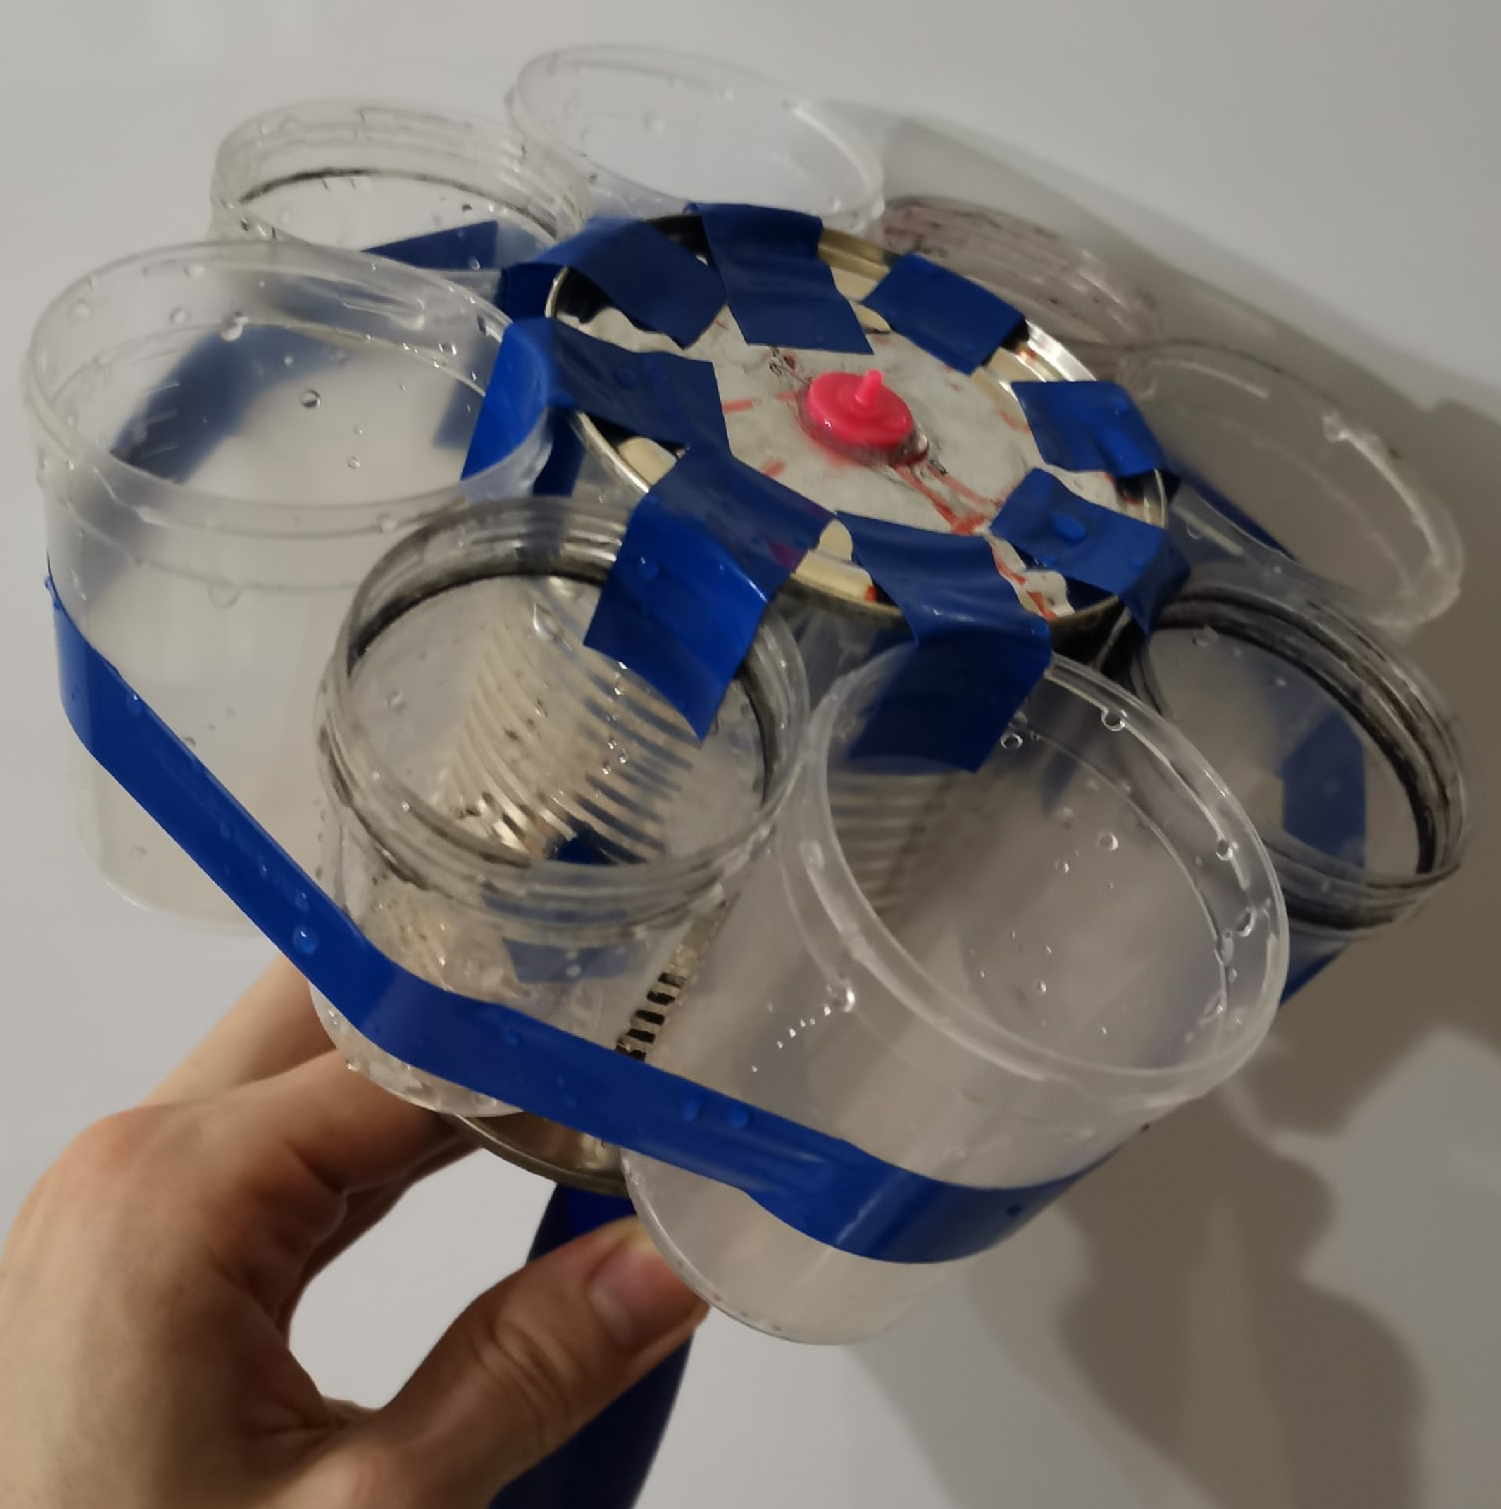
\includegraphics[width = 1\linewidth]{img/equipment.png}
	\end{minipage}
	\hfill
	\begin{minipage}{0.55\linewidth}
		Был проделан эксперимент, в ходе которого было замечено непериодическое движение колеса.

		Однако при попытке снять экспериментальные точки обнаружилась невозможность это проделать из-за неисправности установки.
	\end{minipage}

\end{frame}